\chapter{卷积神经网络理论}
\label{cha:theory}

第一章介绍了卷积神经网络的发展历史,并重点介绍了卷积神经网络的卷积层和池化层的工作原理,用图片展示了这两种神经层的工作原理。第二章介绍了一般神经网络的对训练数据拟合能力以及在测试数据上的泛化能力的理论结果。这一章将介绍卷积神经网络的学习理论内容。

\section{神经网络理论主要问题}
经过数十年的发展,卷积神经网络已经在计算机视觉\cite{krizhevsky2012imagenet}、强化学习\cite{silver2016mastering}、自然语言处理\cite{amari2003handbook}等领域发挥了巨大的作用,例如人脸识别\cite{lawrence1997face,parkhi2015deep},游戏竞技\cite{oh2015action,silver2016mastering},语音识别\cite{abdel2012applying,deng2013new,abdel2014convolutional},语言表示\cite{hu2014convolutional,kalchbrenner2014convolutional},手势识别\cite{molchanov2015hand},在一些应用上的表现甚至已经超过了人类的水平,例如下围棋\cite{silver2016mastering},图像分类\cite{he2016deep},但是对于卷积神经网络拥有惊人表现的原因人们却还没有科学的解释。
\par
近几年,有越来越多的研究者开始对神经网络算法的正确性,有效性进行理论的研究\cite{du2018gradient,allen2019learning,li2018learning,allen2018convergence,brutzkus2017sgd,arora2019fine}。然而,因为卷积神经网络的结构较全连接网络的结构更加复杂,以卷积神经网络理论为主要研究对象的研究还较少。

\par
本文将总结现有文献中的建模方法,以及证明方法,给出现有研究者对卷积神经网络理论研究的主要结果。
\begin{figure}
\centering
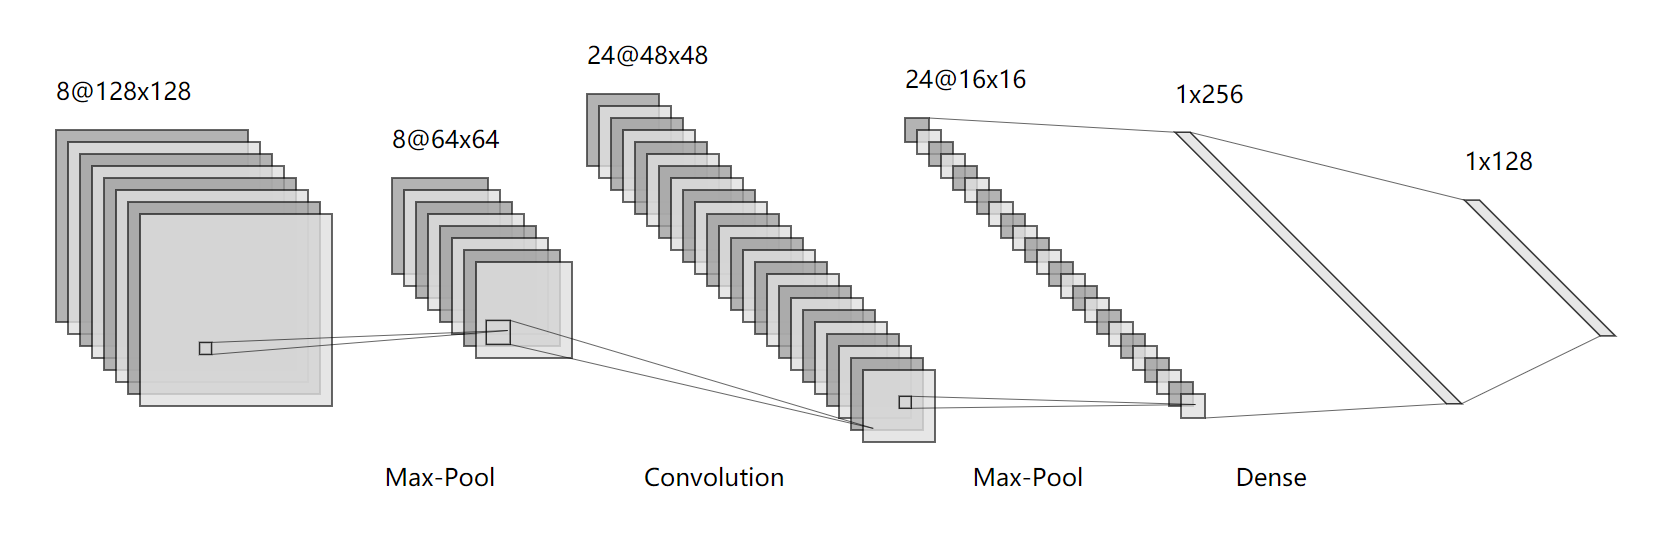
\includegraphics[width=12cm]{./figures/nn.png}
\caption{卷积神经网络实例}
\label{fig:nn}
\end{figure}

\section{卷积神经网络的理论}
\subsection{单层卷积层的神经网络}
\citet{du2018many}考虑了单层卷积层和单层平均池化层以及单层卷积层和单层全连接层组合的两种情况,\citet{du2018many}证明了两种情况下神经网络的均方误差的上下界。下面本文将对其结果进行总结和证明。
\subsubsection{单层卷积层加单层平均池化层}
对于输入$x\in \mathbb{R}^d$,考虑神经网络$F_1: \mathbb{R}^d \mapsto \mathbb{R}$,具体地,
\[
  F_1(x;w) = \sum_{l=0}^{r-1}w^{\top} \mathrm{P}_l^s x
\]
\par
其中$r\approx d/s$,$\mathrm{P}_l^s x=[x_{ls+1},x_{ls+2},\cdots,x_{ls+m}]$,神经网络的结构如图
\begin{figure}
\centering
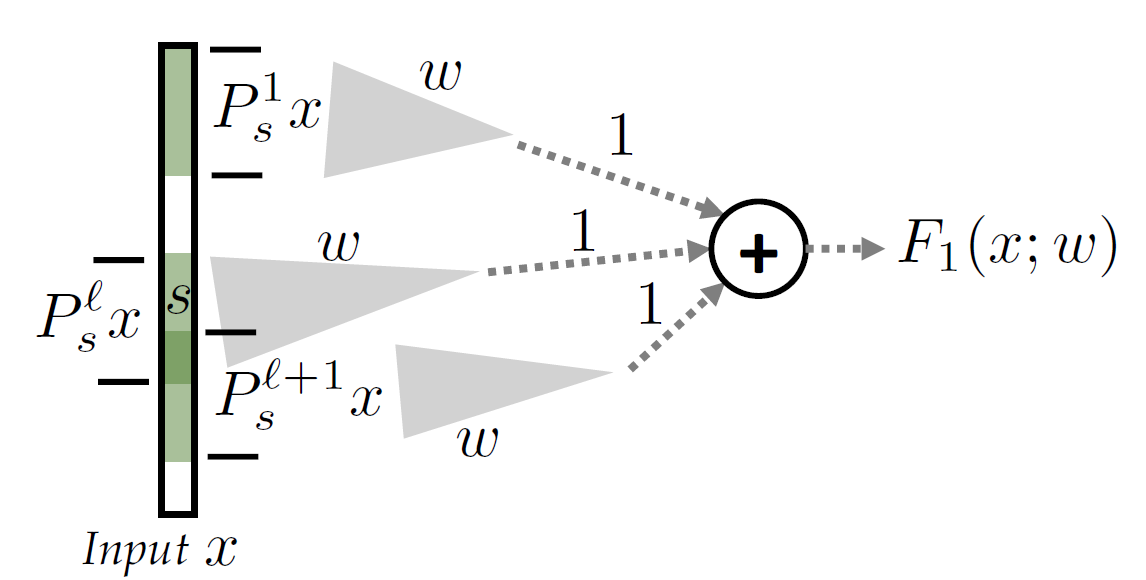
\includegraphics[width=10cm]{./figures/convp.PNG}
\caption{单层卷积层加单层平均池化层}
\label{fig:convp}
\end{figure}
\par
设$\{x_i,y_i\}_{i=1}^n$ 为$n$个训练样本数据,其中$x_i \in \mathbb{R}^d$为输入向量,而$y\in \mathbb{R}$为对应的值。由于实际的数据并不是完全由对应关系决定,而可能会加入噪声,所以这里引入均值为0的噪声,即
\[
  y_i = F_1(x_i;w_0)+\varepsilon_i
\]
\par
其中$\mathbb{E}[\varepsilon_i|x_i] = 0$,输入数据$\{x_i\}_{i=1}^n$从一个未知的分布$\mu$中独立同分布(i.i.d)的取样得到,并且$\mathrm{supp}\mu = \mathbb{R}^d$,即对于$\forall A \in \sigma(\mathbb{R}^d), \mu(A) > 0$,其中$\sigma(\cdot)$为$\sigma-$代数。
\par
对于数据的分布和噪声,有以下的假设:
\begin{assumption}[Sub-Guassian Noise]
存在一个有限常数$\sigma^2< \infty$,满足对$\forall t \in \mathbb{R}, \mathbb{E}[e^{t\varepsilon_i}] \leq e^{\sigma^2t^2/2}$
\end{assumption}
\begin{assumption}
存在一个有限常数$\nu^2< \infty$,满足对$\forall a \in \mathbb{R}^d, \mathbb{E}_\mu x = 0$,有$\mathbb{E}_\mu[\exp\{a^\top x\}]\leq \exp\{\nu^2\|a\|_2^2/2\}$
\end{assumption}
\begin{assumption}
存在正常数$\kappa > 0$,满足$\lambda_{\min}(\mathbb{E}_\mu x x^\top )\geq \kappa$
\end{assumption}
\par
这里的目标是通过训练数据训练神经网络的参数——权重$w$,即
\[
	arg\min_{\hat{w_n}} \sqrt{\mathbb{E}_{x\sim\mu}|F_1(x;\hat{w_n})- F_1(x;w_0)|^2}
\]
\par
这里定义$\mathfrak{M}(n;F_1) = \inf_{\hat{w_n}}\sup_{w_0}\mathbb{E}_{\mu,w_0}[err(\hat{w_n},w_0)]$,其中$err(\hat{w_n},w_0) = \sqrt{\mathbb{E}_{x\sim\mu}|F_1(x;\hat{w_n})- F_1(x;w_0)|^2}$,则有以下的结果,它给出了$\mathfrak{M}(n;F_1)$的一个上界。
\begin{theorem}\label{theo:1}
对于$\delta\in (0,1/2)$和充分大的$n$,对于$\{x_i\}_{i=1}^n$的随机抽样,有$1-\delta$的概率,以下成立
\[
	\mathfrak{M}(n;F_1) \lesssim \sqrt{\frac{\sigma^2 m \log d}{n}}
\]
其中,$\lesssim$表示在不计常数下的$<$。
\end{theorem}
\par
定理~\ref{theo:1}~的证明过程见附录~\ref{pr:1}。

\par
根据定理~\ref{theo:1}~知,所给上界的收敛速率为$O(1/\sqrt{n})$,并且由上界的形式可以知道,所给上界与神经网络的大小没有关系。
\par
以上给出了$\mathfrak{M}$的一个上界,下面将给出其一个下界。
\begin{theorem}\label{theo:2}
假设输入数据$x_i$独立同分布于$\mathcal{N}\sim (0,I)$,假设$\varepsilon_i$独立同分布于$\mathcal{N}(0,\sigma^2)$,则存在一个固定常数$C > 0$满足
\begin{equation}
\mathfrak{M}(n,F_1) \geq C\sqrt{\frac{\sigma^2 m}{n}}
\end{equation}
\end{theorem}



\subsubsection{单层卷积层加单层全连接层}
对于单层卷积层加单层全连接层的神经网路,\citet{du2018many}给出了与单层卷积层单层平均池化层相类似的结果。
\par
对于输入$x\in \mathbb{R}^d$,考虑神经网络$F_2: \mathbb{R}^d \mapsto \mathbb{R}$,具体地,
\[
  F_1(x;w) = \sum_{l=0}^{r-1}a_l w^{\top} \mathrm{P}_l^s x
\]
\par
其中$r\approx d/s$,$\mathrm{P}_l^s x=[x_{ls+1},x_{ls+2},\cdots,x_{ls+m}]$,神经网络的结构如图
\begin{figure}
\centering
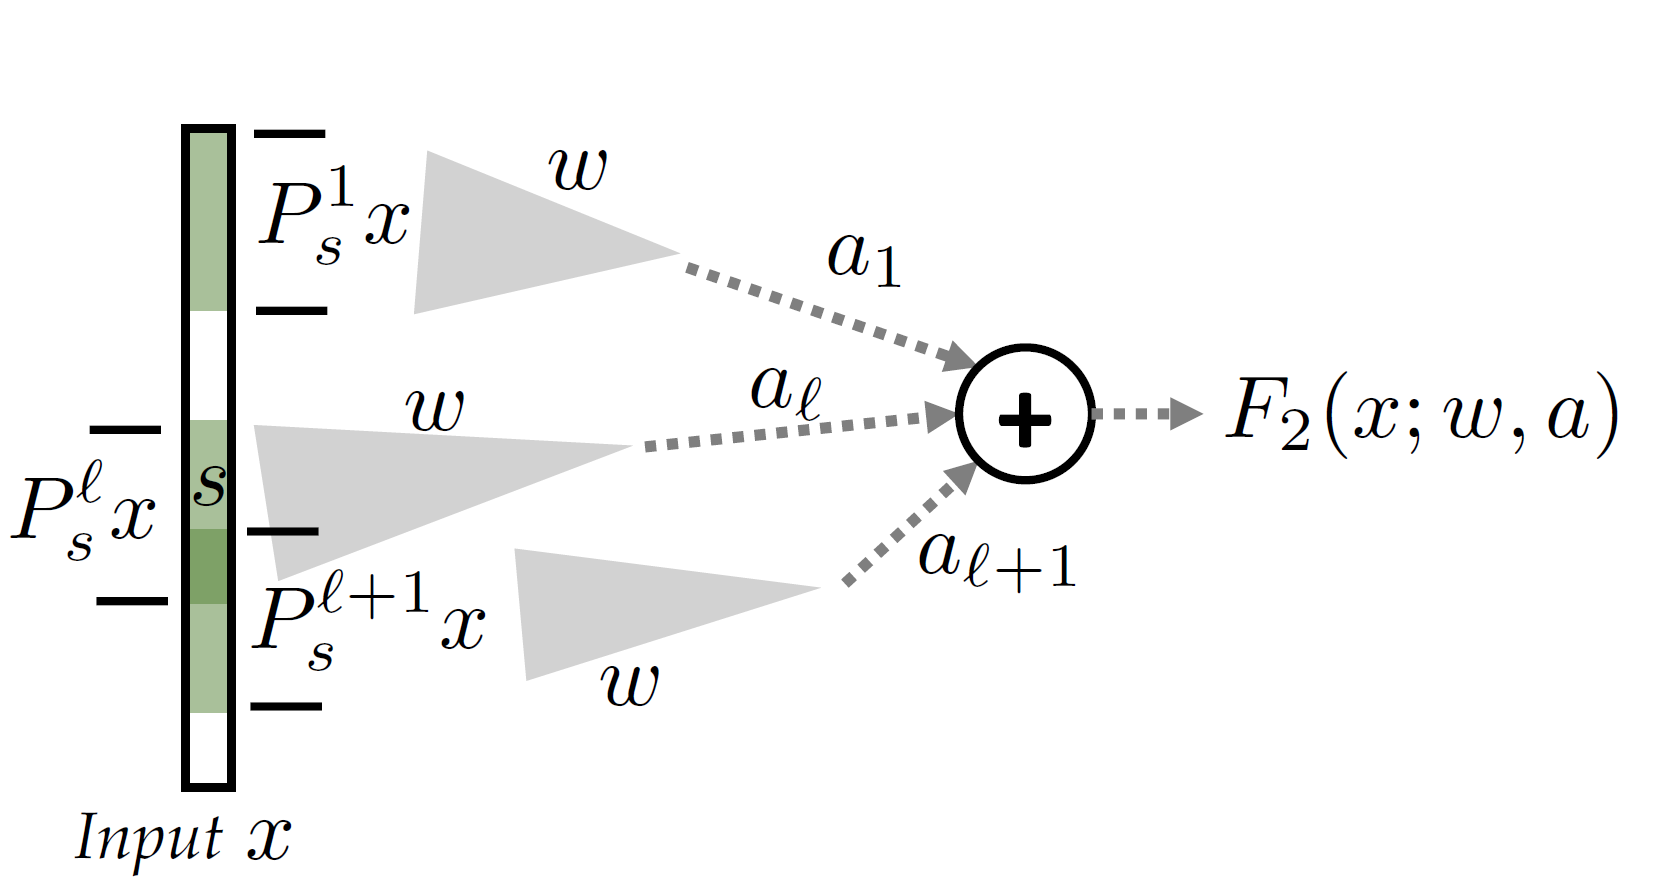
\includegraphics[width=10cm]{./figures/convf.PNG}
\caption{单层卷积层加单层全连接层}
\label{fig:convf}
\end{figure}
\par
设$\{x_i,y_i\}_{i=1}^n$ 为$n$个训练样本数据,在这里有
\[
  y_i = F_2(x_i;w_0)+\varepsilon_i
\]
\par
对于数据的分布和噪声的假设与前一部分一样。
\par
这里定义$\mathfrak{M}(n;F_1) = \inf_{\hat{w_n}}\sup_{w_0}\mathbb{E}_{\mu,w_0}[err(\hat{w_n},w_0)]$,其中$err(\hat{w_n},w_0) = \sqrt{\mathbb{E}_{x\sim\mu}|F_2(x;\hat{w_n})- F_2(x;w_0)|^2}$,则有以下的结果,它给出了$\mathfrak{M}(n;F_2)$的一个上界。
\begin{theorem}\label{theo:3}
对于$\delta\in (0,1/2)$和充分大的$n$,对于$\{x_i\}_{i=1}^n$的随机抽样,有$1-\delta$的概率,以下成立
\[
	\mathfrak{M}(n;F_2) \lesssim \sqrt{\frac{\sigma^2 \min\{d,m+(d/s)\times (m/s)\}\cdot \log d}{n}}
\]
\par
其中,$\lesssim$表示在不计常数下的$<$。
\end{theorem}


\par
根据定理~\ref{theo:3}~知,所给上界的收敛速率为$O(1/\sqrt{n})$,并且由上界的形式可以知道,所给上界与神经网络的大小没有关系。
\par
以上给出了$\mathfrak{M}$的一个上界,下面将给出其一个下界。
\begin{theorem}\label{theo:4}
假设输入数据$x_i$独立同分布于$\mathcal{N}\sim (0,I)$,假设$\varepsilon_i$独立同分布于$\mathcal{N}(0,\sigma^2)$,则存在一个固定常数$C > 0$满足
\begin{equation}
\mathfrak{M}(n,F_2) \geq C\sqrt{\frac{\sigma^2 (m+d/s)}{n}}
\end{equation}
\end{theorem}



\subsection{多层卷积神经网络}
\citet{zhou2018understanding}走的比\citet{du2018many}更远一步,他们考虑了多层卷积神经网络的优化能力和泛化能力,给出了理论的界。下面本文将对其结果进行介绍。
\subsubsection{记号及基本假设}
这里考虑一个$L$层卷积层的卷积神经网络$f(w;X)$,其中$w\in \mathbb{R}^d$为网络的参数,输入数据为$X\in \mathbb{R}^{r_0\times c_0}$,网络的输出为$v\in \mathbb{R}^{d_{l+1}}$,第$i$层卷积层的输入为$X_{i-1} \in \mathbb{R}^{\tilde{r}_{i-1}\times \tilde{c}_{i-1}\times \tilde{d}_{i-1}}$,输出为$X_{i} \in \mathbb{R}^{\tilde{r}_{i}\times \tilde{c}_{i}\times \tilde{d}_{i}}$。第$i$层卷积层进行的计算如下:
\[
 Z_i(:,:,j) = X_{i-1}\circledast W_i^j \in \mathbb{R}^{r_i\times c_i}, \forall j=1,\cdots,d_i
\]
\[
Y_i = \sigma_1(Z_i)\in \mathbb{R}^{r_i\times c_i \times d_i}
\]
\[
 X_i = pool(Y_i) \in \mathbb{R}^{\tilde{r}_i\times \tilde{c}_i \times d_i}
\]
\par
其中,$W_i^j \in \mathbb{R}^{k_i\times k_i \times d_{i-1}}$为第$i$个卷积层的第$j$个卷积核,$\circledast, pool(\cdot), \sigma_1(\cdot)$分别代表卷积操作、池化和sigmoid函数。
\par
整个网络的最后一层为一个全连接层,则最后一层的计算为
\[
u = W_{l+1}x_i \in \mathbb{R}^{d_{l+1}}
\]
\[
v = \sigma_2(u) \in \mathbb{R}^{d_{l+1}}
\]
\par
其中,$x_i = vec(X_i)$为$X_i$的向量化,$\sigma_2(\cdot)$为softmax函数。
\par
这里我们考虑的损失函数为
\[
	\tilde{Q}_n(w) = \frac{1}{n} l(f(w;X_i), y_i)
\]
\par
其中$l(f(w;X),y) = \frac{1}{2}\|v-y\|_2^2$,同时,模型在整体分布上的误差为
\[
	Q(w) = \mathbb{E}_{X,y \sim \mathcal{D}} l(f(w;X),y)
\]
\par
其中$\mathcal{D}$为输入数据的分布。
\par
为了证明$\tilde{Q}_n(w)$可以收敛到$Q(w)$,这里需要先引入两个基本假设。
\par
第一条假设神经网络的权重为有界的。
\begin{assumption}
第$i$层卷积层的第$j$个卷积核$W_i^j\in\mathbb{R}^{k_i\times k_i \times d_{i-1}}$和$W_{L+1}\in \mathbb{R}^{d_{L+1}\times \tilde{r_L}\tilde{c_L}d_L}$均有界
\[
\|W_i^j\|_F \leq b_i (1\leq j\leq d_i; 1\leq i \leq L )
\]
\[
\|W_{L+1}\|_F \leq b_{L+1}
\]
其中$b_i, 1\leq i \leq L+1$为有限正常数。
\end{assumption}
\par
这里,$\|\cdot\|_F$为Frobenius范数。
\par
在训练神经网络之后得到的参数往往都是非满秩的,所以作以下的假设
\begin{assumption}
设$\tilde{W}_i = [vec(W_i^1), vec(W_i^2),\cdots, vec(W_i^{d_i})]$,则假设$rank(\tilde{W}_i) \leq a_i, rank(W_{L+1}\leq a_{L+1})$.
\end{assumption}

\subsubsection{理论结果}
\par
基于以上的两个假设,有以下的结果
\begin{lemma}
在以上两个假设成立的条件下,如果$n\geq c_{f^\prime}L^2(b_{L+1}+\sum_{i=1}^L d_i b_i)^2 \max_i \sqrt{r_ic_i}/(\theta \varrho \epsilon^2)$,其中$c_{f^\prime}$为一个常数,则以概率$1-\epsilon$,有
\begin{equation}
\sup_{w\in \Omega} |\tilde{Q}_n(w)-Q(w)|\leq \sqrt{\frac{\theta \varrho +\log(4/\epsilon)}{2n}}
\end{equation}
\par
其中$\theta = a_{L+1}(d_{L+1}+\tilde{r}_L\tilde{c}_Ld_L+1)+\sum_{i=1}^L a_i(k_i^2d_{i-1}+d_i+1),  \varrho = \sum_{i=1}^L \log\big(\frac{\sqrt{d_i}b_i(k_i-s_i+1)}{4p}\big)+\log(b_{L+1}) + \log{\frac{n}{128p^2}}$
\end{lemma}
\par
基于以上的引理,有以下的结果
\begin{theorem}\label{theo:2:1}
以概率$1-\epsilon$有
\[
\mathbb{E}_{(X,y)\sim \mathcal{D}}|\mathbb{E}_{\mathcal{A}}(Q(\tilde{w}) - \tilde{Q}_n(\tilde(w)))| \leq \sqrt{\frac{\theta \varrho + \log(4/\epsilon)}{2n}}
\]
\end{theorem}

\par
定理~\ref{theo:2:1}~说明了泛化误差的下降速度为$O(1/\sqrt{n})$。由于$\theta$代表了神经网络参数集的自由度数,它与神经网络的大小有关,为了降低泛化误差,需要有更多的训练数据。对于参数$\varrho$,其中的参数$k_1,s_i$都对神经网络的泛化误差有影响。$k_i$越大,则网络中的参数越多,训练网络更加困难,使得模型的泛化误差较大;而$s_i$越大,则网络的复杂度越低,训练越容易,模型的泛化误差越小。同时,$\theta, \varrho$中都含有$d_i$,这使得越宽的网络需要越多的训练数据进行训练,因为$d_i$越大,网络的参数越多,从而$\theta$增大。

\par
在给出泛化误差的控制之后,进一步考察模型是否可以达到训练过程的收敛,以下将分几步说明。

\begin{theorem}\label{theo:2:2}
在假设成立的情形下,经验梯度一致收敛,即,存在常数$c_{g^\prime}, c_g$,满足当$n \geq c_{g^\prime}\frac{L^2 b_{L+1}^2(b_{L+1}+\sum_{i=1}^Ld_ib_i)^2(r_0d_0c_0)^4}{d_0^4b_1^8(d\log(6)+\theta\varrho)\epsilon^2\max_i(r_ic_i)}$时,有
\[
\sup_{w\in \Omega} \|\nabla_w \tilde{Q}_n(w)-\nabla_wQ(w)\|_2\leq c_g \beta \sqrt{\frac{2d+\theta\varrho+\log(4/\epsilon)}{2n}}
\]
\par
至少以概率$1-\epsilon$成立,其中
\[
\beta = [\frac{r_Lc_Ld_L}{8p^2}+\sum_{i=1}^L\frac{b_{L+1}^2d_{i-1}}{8p^2b_i^2d_i}r_{i-1}c_{i-1}\Pi_{j=i}^l\frac{d_jb_j^2(k_j-s_j+1)^2}{16p^2}]^{1/2}
\]
\[
d = \tilde{r}_L\tilde{c}_L d_Ld_{L+1}+\sum_{i=1}^L k_i^2d_{i-1}d_i
\]
\end{theorem}
\par
从以上定理可见,经验梯度以$O(1/\sqrt{n})$收敛。下面的一个推论说明了$\nabla \tilde{Q}$和$\nabla Q_n$之间的关系。
\begin{corollary}\label{coro:2:1}
设定理~\ref{theo:2:2}~成立,并且$n \geq (d\varrho +\log(4/epsilon))\beta^2\epsilon$。则若由最小化经验误差得到的$\tilde{w}$使得$\|\nabla \tilde{Q}_n(\tilde{w})\|_2^2 \leq \epsilon$,则有$\|\nabla Q(\tilde{w})\|_2^2 \leq 4\epsilon$以至少概率$1-\epsilon$成立。
\end{corollary}
\par
推论~\ref{coro:2:1}~说明$\min \tilde{Q}_n$对应的最优解$\tilde{w}$和$\min Q$对应的最优解$w^*$十分接近,这说明了神经网络的有效性。
\par
为了更加准确的说明两者之间的关系,下面进一步考察驻点之间的差距。
\par
首先引入非退化驻点的概念。
\begin{definition}
驻点$w$称为非退化驻点,若
\[
\inf_i |\lambda_i(\nabla^2 Q(w))| \geq \xi 
\]
\par
其中$\xi$为一个正常数,$\lambda_i(\nabla^2 Q(w))$为Hessian矩阵$\nabla^2 Q(w)$的第$i$个特征值。
\par
驻点$w$称为鞍点,若$\nabla^2 Q(w)$的最小的特征值为负。
\end{definition}
\par
当$Q(w)$有一个非退化的驻点时,有以下结果。
\begin{theorem}\label{theo:2:3}
当$n \geq c_h \max(\frac{d+\theta\varrho}{\xi^2},\frac{L^2b_{L+1}^2(b_{L+1}+\sum_{i=1}^Ld_ib_i)^2(r_0c_0d_0)^4}{d_0^4 b_1^8d\varrho \epsilon^2\max_i(r_ic_i)})$,其中$c_h$为一常数。对$k\in\{1.\cdots,m\}$,存在$\tilde{Q}_n(w)$的非退化驻点$w_n^k$以至少概率$1-\epsilon$与$Q(w)$的非退化驻点$w_k$唯一地对应,同时,至少以概率$1-\epsilon$有
\[
\|w_n^k - w_k\|_2 \leq \frac{2c_g \beta}{\xi}\sqrt{\frac{2d+\theta\varrho+\log(4/\epsilon)}{2n}}\quad 1\leq k \leq m
\]

\end{theorem}

\par
定理~\ref{theo:2:3}~说明,当训练样本的数量足够大时,$w_n^k$与$w_k$存在一一对应,并且二者之间的距离被$O(1/\sqrt{n})$控制住。对于退化驻点,由于Hessian矩阵的特征值中有0,使得它们之间没有一一对应。

\par
现在考虑另一类损失函数,具体的,设$l:\mathbb{R}\times \mathbb{R} \rightarrow [0,1]$是满足对所有的$y, l(\cdot,y)$为$\lambda-$Lipschitz的。输入数据为$x \in \mathbb{R}^{d\times d \times c}$,卷积层的卷积核为$K^i \in \mathbb{R}^{k\times k \times c\times c}, i\in\{1,\cdots,L\}$,卷积核的初始值为$K_0^i$,设$op(K^i)$为$K^i$的算子矩阵\cite{sedghi2018singular},且$\|op(K^i_0)\|_2 = 1$,定义卷积核与初始值之间的距离为$\|K-K_0\|_\sigma = \sum_{i=1}^L\|op(K^i) - op(K_0^i)\|_2$,定义$F_\beta = \{f_K : \|K-K_0\|+\sigma \leq \beta\}$,则有以下的结果,结果属于\citet{long2019size}。

\begin{theorem}
对任意的$\eta > 0$,存在$C>0$使得对任意$\beta, \delta > 0, \lambda \geq 1$,以及任意的$\mathbb{R}^{d\times d \times c}\times \mathbb{R}$的乘积$\sigma-$代数上的联合概率分布测度$P$,$\{(x_i, y_i)\}_{i=1}^n$独立同分布于$P$,则对$\forall f\in F_\beta$以至少概率$1-\delta$有
\[
\mathbb{E}_{z\sim P}[l_f(x,y)] \leq (1+\eta)\mathbb{E}_S [l_f] + \frac{C(Lk^2c^2(\beta+\log(\lambda n)) + \log(1/\delta))}{n}
\]
\par
并且,$\beta \geq 5$时,有
\[
\mathbb{E}_{z\sim P}[l_f(x,y)] \leq \mathbb{E}_S[l_f]+C\sqrt{\frac{Lk^2c^2(\beta + \log(\lambda))+\log(1/\delta)}{n}}
\]
\par
当$\beta < 5$时,有
\[
\mathbb{E}_{z\sim P}[l_f(z)] \leq \mathbb{E}_S[l_f]+ C\big(\beta \lambda \sqrt{Lk^2c^2/n} + \sqrt{\frac{\log(1/\delta)}{n}}\big)
\]
\par
其中$l_f(x,y) = l(f(x),y)$
\end{theorem}

\par
上述定理给出了对CNN的泛化能力的一个估计,利用训练误差控制住了CNN在测试集上的误差。
